\documentclass[tikz,border=1.35mm]{standalone}

\definecolor{fvmadaptedge}{HTML}{8A7E7E}

\definecolor{splitred}{HTML}{AF2525}
\definecolor{splitgreen}{HTML}{0E8814}

% One quadrilateral child face highlighted inside a split quadrilateral.
% Coordinates are in millimeters; y=-1mm keeps the SVG-style origin at top left.
\begin{document}
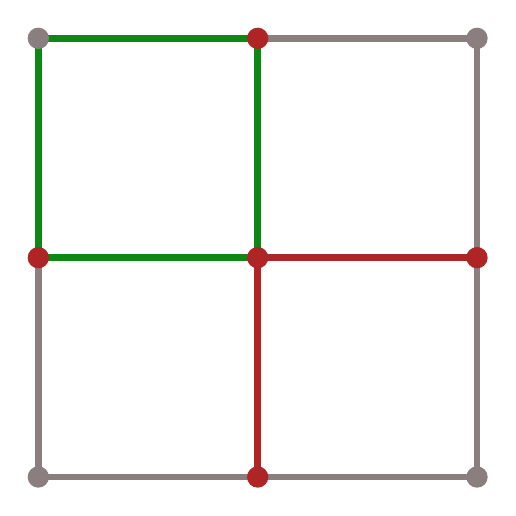
\begin{tikzpicture}[
  x=1mm,
  y=-1mm,
  line join=round,
  edge/.style={draw=fvmadaptedge,line width=0.865mm},
  splitline/.style={draw=splitred,line width=0.865mm},
  greenedge/.style={draw=splitgreen,line width=0.865mm}
]
  % Match the original artwork frame before the standalone border is applied.
  \useasboundingbox (0,0) rectangle (58.419,58.419);

  % Original quadrilateral vertices plus split-created edge midpoints and face center.
  \coordinate (topLeft) at (1.353,1.353);
  \coordinate (topRight) at (57.067,1.353);
  \coordinate (bottomRight) at (57.067,57.067);
  \coordinate (bottomLeft) at (1.353,57.067);
  \coordinate (topMid) at (29.210,1.353);
  \coordinate (rightMid) at (57.067,29.210);
  \coordinate (bottomMid) at (29.210,57.067);
  \coordinate (leftMid) at (1.353,29.210);
  \coordinate (center) at (29.210,29.210);

  % Draw the original boundary in #8a7e7e, then the split-node connections in red.
  \draw[edge] (topLeft) rectangle (bottomRight);
  \draw[splitline] (topMid) -- (center) -- (bottomMid);
  \draw[splitline] (leftMid) -- (center) -- (rightMid);

  % Green edges indicate the selected upper-left quadrilateral child face.
  \draw[greenedge] (topLeft) -- (topMid) -- (center) -- (leftMid) -- cycle;

  % Original vertices are #8a7e7e.
  \fill[fvmadaptedge] (topLeft) circle[radius=1.353mm];
  \fill[fvmadaptedge] (topRight) circle[radius=1.353mm];
  \fill[fvmadaptedge] (bottomRight) circle[radius=1.353mm];
  \fill[fvmadaptedge] (bottomLeft) circle[radius=1.353mm];

  % Split-created edge and face nodes are red.
  \fill[splitred] (topMid) circle[radius=1.353mm];
  \fill[splitred] (rightMid) circle[radius=1.353mm];
  \fill[splitred] (bottomMid) circle[radius=1.353mm];
  \fill[splitred] (leftMid) circle[radius=1.353mm];
  \fill[splitred] (center) circle[radius=1.353mm];
\end{tikzpicture}
\end{document}
